%!TeX encoding = UTF-8
%!TeX spellcheck = es_ES
%!TEX root=../../main.tex

\epigraph{Quien desconoce el motivo de las normas está condenado a respetarlas.}{Valérie Tasso}

\begin{abstract}
Ya hemos hablado de las normas y su porque general. En este capitulo veremos una serie de reglas que siempre se deberan cumplir si o si. Veremos que son muy logicas y basadas en cuestiones tecnicas sin ser muy arbirarias.
\end{abstract}

\section{Introducción}
Hemos visto que a nivel legal siempre hemos recalcado al menos tres tipos de normas:
\begin{itemize}
	\item \textbf{Estructurales}: Son las normas que dictan cuanto peso soporta una habitacion y lo que debe pesar nuestra maqueta.
	\item \textbf{Electricas}: Como debe de ser la instalacion electrica para ser segura.
	\item \textbf{Sanitarias}: En caso de hacer un negocio los requisitos sanitarios y de seguridad que deben segir.
\end{itemize}
De las cuales, no siempre vamos a crear un negocio, por lo que solamente nos centraremos en las dos primeras.

Asi mismo estas dos normativas legales se han ido creando en el tiempo debido a accidentes y su objetivo es minimizar el riesgo a las personas.
Su no cumpliemento, ademas de una multa, puede ocasionar graves daños personales (incendios, derrumbes,\dots).

\section{Estado del arte}
Cada pais tiene un reglamento de como se debe construir una casa y que pesos puede soportar un edificio. Y lo mas sorprendente, donde puede o no puede instalarse un armario.

Igualemnte para la instalacion electrica, cada pais tiene su reglamento que indica que cables se pueden usar y donde colocarlos.
\subsection{Estructura y Pesos}
Los libros y la ropa pesan mucho más de lo que nos pensamos, y si no que les pregunten a las lineas aereas. Si nos fijamos cuidadosamente, las paredes para armarios se situan entre columnas, lo que hara que el peso recaiga sobre una viga y no sobre el centro de una habitacion.

Asi mismo, una reforma del baño hay que tener cuidado por que la zona de la bañera esta reforzada para poder soportar el peso de varios adultos y el agua que pueda entrar, si no fuera asi, las escenas donde cae una bañera se verian más que en el cine.

Cuando se compra una casa, al nuevo dueño se le deberia incluir un manual donde se indiquen los kilos soportados por metro cuadrado y donde colocar los armarios pesados.

No poner el peso en el lugar correcto, o ubicar más peso donde no se deberia, hace que corramos el riesgo de que el suelo se caiga. Y nuestro suelo es el techo del vecino de abajo.
\subsection{Instalacion Electrica}
El reglamento de las instalaciones electricas varia de pais a pais, pero todos van a tener unos apartados similares:
\begin{itemize}
	\item \textbf{Tipos de cables}: Segun el Amperaje que debe soportar el circuito, que cable usar (seccion y materiales aislantes)
	\item \textbf{Voltajes}: Voltajes del sistema, normalmente si es 110V o 220V y que amperajes maximos deben ir por cada circuito, 16A o 20A, pòr lo general\footnote{Se recomienda revisar en su pais, lo que dice concretamente la normativa}.
	\item \textbf{Elementos fijos}: Como son los enchufes, los interruptores, tanto desde el punto de vista mecanico (forma y materiales), como de su numero, y ubiocacion en una habitacion. 
	\item \textbf{Canalizaciones}: Como deben ser los tubos que llevan los conductures, puesto que entre enchufe y enchufe, el cable debe ir en un tubo, no puede ir al aire. La norma dice tambien cuantos conectores pueden ir por un tubo concreto.
	\item \textbf{Distancias de seguridad}: Relacionado con la ubicacion de los elementos fijos  pero referido a distancias minimas de seguridad para no causar problemas con otros elementos, como fuentes de agua.
\end{itemize}
Estos temas son los mas tipicos que nos podremos enconctrar, sobre todo relacionados con un piso normal. Pero la norma debe abacar todo tipo de viviendas.

Desde un punto de vista tecnico no seguir estas reglas pueden producir tres tipos de problemas:
\begin{itemize}
	\item \textbf{Chispas}: Cuando dos conductores con cargas(voltajes, resumidamente) diferentes se acercan mucho entre si, salta una chispa entre ellos. Esta chispa puede producir un incendio si toca algun material inflamable.
	\item \textbf{Calor}: La corriente que pasa por un conductor lo calienta. Segun la seccion se calentara más o menos (a misma corriente). La normativa indica que conductor se debe usar segun la corriente máxima que pasa por el. Tambien se puede leer al reves, segun la seccion como mucho puede pasar tanta corriente. 

Esta combinacion seccion/corriente es la que hace que el conductor se caliente como mucho a 70 grados, y que se considera segura para los aislantes usados. Si se utilzar para más corriente se corre el riesgo de que se caliente más, ya de por si este calor tiene la posibilidad de iniciar un fuego. Pero ademas este calor extra hace correr el riesgo de que se funda el aislante y exponga un conductor a otros de diferente voltaje, pudiendo provocar una chispa.
	\item \textbf{Descargas no deseadas}: Toda instalacion tiene dos cables, Neutro (sin voltaje) y Vivo (con voltaje Alterno). Pero que no tenga voltaje, no significa que no lleve corriente. En la practica se puede decir\footnote{Simil para entender, la realidad es un poco más complicada} que la corriente nos viene por el cable ``vivo'', la usamos en nuestro electrodomestico y vuelve por ``neutro'' a la central electrica. A veces, por una mala instalacion o un fallo en el electrodomestico, esa corriente vuelve pasando por el usuario del mismo pudiendo causar un paro cardiaco u otros problemas.
\end{itemize}
\subsection{Instalacion electrica Tipica}
La instlacion tipica de una casa empieza con la conexion del contador al interruptor general. Luego de ahi se va a varios intrruptores de circuito y luego cada circuito va a una o varias cajas de empalmes. Suele a ver una caja por habitacion y de ahi se unen los conductores de los enchues de la habitacion. 

Dibujo mostrando esto

Las normativas indican cuantos enchufes pueden ir a un circuito, si hay circuitos para iluminacion, o para electrodomesticos especificos (como aires acondicinados, hornos, neveras,\dots)

Para complicar un poco más las cosas, las empresas nos cobran por KiloWatios, pero las limitiaciones son por Amperios. Por suerte hay una relacion sencilla.
\section{Peso Máxmimo de la maqueta}
Podemos considerar que en una construccion moderna, va a ser muy dificil que una maqueta de tren (grande superficie plana con "poco" volumen) supere el maximo de ocupacion de una casa, a menos que usemos la parte inferior para almacenaje de objetos pesados.

Todas las construcciones deben soportar una sobrecarga mucho mayor de 150 Kg por Metro cuadrado\footnote{En España es de 300 segun normativa de 2020, 200 en construcciones anteriors a 1965}. Eso significa poner más de 150 KG en cada cuadrado de un metro de largo. En una habitacion de 10m2 serian poner 1500 KG o el equivalente a 20 personas promedio. 

En caso de duda se puede medir los m2 en planta que ocupa la maqueta y multiplcar por 100KG si pesa menos, estaremos tranquilos, si pesa más limitaremos el contenido interior.

\section{Consumo de la maqueta}
En esta seccion vamos a ver como calcular cuantos Watios consume nuestra maqueta y ver si nuestra instalacion lo soporta.

Las Formulas son simplificaciones con error a mayor. Un ingeniero electrico podra ver que hay algunos errores pero estas simlificaciones estan pensadas para que un usuario calcule mas Watios consumidos y asi estar en zona segura.
\subsection{¿Cuantos Boosters?}
Para saber cuanto consume nuestra maqueta tenemos que saber cuantos booster necesitamos, estos se calculan en funcion de las maquinas (decoders) que vamos hacer correr a la vez en nuestra maqueta. Mirar en documentaciones cuanto consumen y sumar por este lado. Luego veremos cuanto puede suministrar nuestra central y los boosters que tengamos y aseguranos que esta suma es superior.

$A_{central} + \sum_{n=1}^{nBoosters}A_{Booster}(n) \geq \sum_{i=1}^{nDecoders}A_{Decoders}(i)$

En este punto, no vamos a entrar en como saber cuanto nos consumen los trenes en funcion de lo que estan haciendo y nos bastara aplicar la regla simple de esperar 0.5 amperios por maquina. 

$A_{central} + \sum_{n=1}^{nBoosters}A_{Booster}(n) \gg 0.5\times nDecoders $

Como los Decoders nos dicen cuantos ameperios necesitan y los Booster cuantos Amperios pueden suministrar, hasta este punto es facil, solo es cuestion de usar el Booster que nos de los suficientes y estos facilmente los encontramos de 2, 3, 10, 15, 20,\dots.
\subsection{¿Cuanto nos sonsumen nuestros boosters?}
El siguente problema es saber cuanta energia vamos a pedir a nuestra instalacion. 
Si nos fijamos en los enchufes tipicos\footnote{O en las alargaderas}, veremos que solo soportan 16A como mucho\footnote{Segun el fabricante, Recomendamods no meter más de 12A en algunas bases multiples\dots}. Eso nos puede llevar a pensar que no podemos tener Boosters de más de 15A, pero alguno hay de 20A. ¿Como puede ser esto posible?\dots. Para simplificar el texto, vamos a suponer que tenemos un Booster de 10 Amperios y 15 Voltios de salida.

La razon es que, desde el punto de vista de consumo, un Amperio a 15V no es lo mismo que a 220V. Lo importante es energia utilizada, que se mide en Julios y se calcula como la integral de la potencia instantana durante un periodo de tiempo t. Si el consumo es constante se puede simplificar en la multiplicacion de la potencia por el tiempo.

$ E= \int_{i}^{t}{p(i)dt} \approx P\cdot t$ 

La potencia se mide en Watios, y si la multiplicamos por el tiempo de medida, tenenos la energia usada en ese periodo\footnote{En el S.I. Watios Segundo, o Julios}. Si nuestro periodo lo medimos en horas, podemos multiplicar directamente los Watios por esas horas y tenemos la energia en Watios Hora, que es lo que nos cobran\footnote{Las compañias cobran por KiloWatioHora, pero solo es dividir por 1000}. Lo bueno de usar esta unidad es que nos permite entender una cosa, si nuestra consumo es 10 Watios-Hora nos da igual que hayan sido 10 Watios en una hora que 1 W en 10 horas, el resultado es el mismo.

Volviendo a los boosters, se puede decir que son un sistema transformador de energia, de 220V en alterna a 15V en continua por lo que la energia de salida (10 Amperios a 15 Voltios) debe ser la misma que de entrada (X Amperios a 220 Voltios). En la practica van a haber perdidas\footnote{En forma de calor} por lo que la energia de entrada sera superior. Como regla general, podemos decir que perdemos un 20%

$E_{entrada} = E_{salida} + E_{perdida}$

$E_{entrada} > E_{salida}$

$E_{entrada} \approx 1.20 \cdot E_{salida}$

Pero esta energia de entrada debe ser en el mismo periodo y ademas para saber cuanto puede consumir nuestra maqueta, hay que ponerse en el peor caso. Siendo este que el booster este dando al maximo durante todo el tiempo\footnote{Si hacemos nuestros calculos seguros para ese caso, sabremos que sera seguro para la realidad, ya que siempre sera menor nuestro consumo}, lo que es consumo constante asi que podemos sustuir por la multiplicacion y simplificar el termino t en la equivalencia

$E_{entrada} \approx 1.20 \cdot E_{salida}$

$P{entrada}\cdot t \approx 1.20 \cdot P_{salida} \cdot t$

$P_{entrada} \approx 1.20 \cdot P_{salida}$

Lo que quiere decir que nos podemos fijar solo en los Watios y olvidarnos del tiempo.

Pero como calculamos los Watios de nuestros boosters, pues la potencia en un momento dado es la multiplicacion del voltaje por la corriente (Voltios por Amperios). En corriente Continua, siempre tenemos los mismos voltios y la misma corriente, por lo que se simplifican los calculos para calcular la potencia real:

$p(i) = v(i) \cdot a(i)$

$P = V \cdot A$

En corriente alterna, donde el voltaje y la corriente forman una señal periodica que se repite un tiempo, el calculo es mas complicado y se hace la media sobre el tiempo de cada periodo. Por suerte para las señales tipicas se han calculado simplificaciones con dos factores, uno de forma y otro de potencia.

$ P_{ac} =\frac{1}{T} \int_{i=0}^{i=T}{v(i)\cdot a(i)\cdot dt}$

$ P_{ac} = V \cdot A \cdot F_{forma} \cdot F_{potencia} $

Ambos factores siempre son menores o iguales a 1 y dependen del tipo de señal (Sinosuidal, triangular, cuadrada,...) y del desfase entre corriente y volataje. Por suerte para el factor de forma se tiene ya calculado y el Factor de potencia en los sistemas domesticos debe ser cercano a 1. Para las ondas sinusoidales es $\frac{1}{\sqrt{2}} \approx 0.707$, conociendo este dato se puede asignar un factor de potencia equivalente de tal forma que de $\frac{1}{2}$

$F_{forma} \cdot F_{potencia} \approx  \frac{1}{2} $

Dicho esto ya podemos ver tres formas de como saber cuantos amperios circularan por nuestro circuito electrico

\subsubsection{La Matematica}
Sabemos que la energia de entrada debe ser la de salida, pero podemos simplificar a la potencia de entrada debe ser la misma ya que es siempre en la mismo tiempo. 

$ E_{entrada} = E_{salida} $

$ P_{entrada} = P_{salida} + P_{perdida} $ (teniendo en cuenta perdidas)

$ P_{entrada} = 1.20 \cdot P_{salida} $

$ V_{ac} \cdot A_{ac} \cdot F_{forma} \cdot F_{potencia} = 1.20 \cdot V_{salida}\cdot A_{salida}$
$ A_{ac} = \frac{1.20 \cdot V_{salida}\cdot A_{salida}}{V_{ac} \cdot F_{forma} \cdot F_{potencia}} $ (Reorganizando)

$ A_{ac} = \frac{1.20}{F_{forma} \cdot F_{potencia}} \cdot\frac{V_{salida} }{V_{ac}} \cdot A_{salida} $

Hemos añadido las perdidas, puesto que la informacion que tenemos de la potencia de salida, es la potencia que se entrega a las vias, no la que  el mismo booster necesite para sus operaciones.

Ademas hemos reorganizado los terminos para encontrarnos con dos factores sobre el amperaje de salida:

$\frac{1.20}{F_{forma} \cdot F_{potencia}}$ y $\frac{V_{salida} }{V_{ac}} $

El primero es un factor que depende de las perdidas  y el segundo segun la relacion entre los voltajes.

Si sustimos la informacion que tenemos nos queda:

$A_{ac} =  \frac{1.20}{0.5}\cdot\frac{15}{220}{10}$

$A_{ac} \approx  2,40\cdot\frac{7}{100}\cdot {10}$

$A_{ac} \approx \frac{17}{100}\cdot{10} \approx 0,17\cdot 10 \approx 1.7$

Si se revisan los calculos se podra observar que esta cifra obtenida es ligeramente mayor al resutaldo ``real''. Ademas el primer factor depende de las perdidas y de que el transformador tenga un factor de potencia tal que duplique ese 1.20.
Estos valores, han sido escogidos suponiendo una mal diseño del transformador que de la corriente al booster. En la practica para poder venderse como domestico, estos valores deberan ser más peqeños y ese factor estara más cerca del 1.50 que el 2.40 obtenido.

Estos calculos habra que realizarlos cada voltaje de salida y de entrada (en caso de no ser 220V, como en europa). Por ejemplo para 18V, nuestros 10A se convierten en 2A en 220V y 4A en 110V.

Nota: Los voltajes recomenados para H0 y N son 16 y 12V, respectivamente. por lo que 18V estaria por encima de las recomenaciones\footnote{Otras escalas pueden usarlo, recomendamos rehacer estos calculos a necesidad}.

En este metodo, podemos ajustarnos más al tope que puede suministrarnos\footnote{Repitiendolos para los datos concretos y siempre dejando al menos 0.5A como margen}, con los datos de los calculos podriamos poner 9 Boosters y aun nos sobrarian 0,7 Amperios\footnote{Aunque esto no deja espacio para otras cosas, como iluminacion de la habitacion, ordenadores, accesorios,...}. Y eso serian 90 amperios a 15V con lo que podriamos tener 180 locomotoras al maximo a la vez, con lo que no estariamos hablando de una maqueta pequeña.

\subsubsection{La rapida}

El objetivo de estos calculos es saber cuantos booster podemos poner en nuestro circuito de casa. Lo que quiere decir que si nos equivocamos en el consumo por arriba, suponiendo que nos consume más de lo que luego consumen realmente, y aun asi no alcanzamos el limite que nos puede suministrar, no estaremos poniendo en peligro la instalacion.

Por lo que podemos hacer un calculo rapido suponiendo que cada Amperio de salida nos consume 0.2 Amperios de entrada, o que es lo mismo, dividir por 5. Esto para el caso de 220V, para 110 bastaria 0,4 Amperios o dividir por 2.5. 

Este calculo rapido vemos que nos sirve para los voltajes recomendados de H0 y de N, incluso llendonos a 18V.

En todo caso si utilizamos este metodo se deberia dejar al menos 1A margen

Con este sistema, por cada Booster de 10A necesitamos 2Amperios, por lo que en nuestra liena de 16A podriamos poner 7, dejando de margen 2A\footnote{8 nos deja sin margen}.

\subsubsection{La tecnica}
Si nos fijamos en las fichas tecnicas de los transformadores que se usan en los boosters, vermos que hay una tabla que dice el voltaje y los amperios de salida y los de entrada.

(Foto de un transformador)

Lo bueno de estos datos es que ya tienen en cuenta las posibles perdidas y los factores de potencia, por lo que los datos son más reales.

En la foto incluida se puede ver que nos produce XXA y necesitamos YYY Amperios en corriente alterna, Si hacemos los calculos matematicos vemos que nos produce un error de ZZZ, y ahora podemos tener

\subsubsection{Pensar en Watios}

Otra forma de calcular lo que nos va a consumir es pensar en Watios. Si sabemos el voltaje y su corriente maxima, podemos tener en cuenta las formulas, perdidas y demas podemos decir:

$P_{ac}=V\cdot A \cdot F_{potencia}\cdot P_{forma}=220 \cdot 16 \cdot \frac{1}{2} = 1760 \approx 1800W$

$P_{salida}= V\cdot A +P_{perdidas}\approx 1.20\cdot V\cdot A =15 \cdot 10 \cdot 1.20=180W$

A partir de aqui es cuestion de pasar a W todos los dispositivos y sumar hasta que nos llege a 1800W.

Nota: ¿Como es posible que haya planchas de más 2.200 W? 

Esto es muy sencillo, hemos realizado los calculos suponiendo que el factor de forma y de potencia nos de como combinados 0.5 y ya hemos dicho que estamos considerando una situacion mala que nos limita los Watios que nos suministra la instalacion. Una plancha es una carga resistiva cuyo factor de potencia es 1\footnote{O tan cercano que se simplifca a 1} en ese caso, $P_{forma}=\frac{1}{\sqrt{2}}\approx=0.707$. A 220V nos suministra unos 2500W, pero ademas, para asegurar un minimo las compañias envian la coriente a 240V, en esta situacion el maximo es 2800W.

Esto suponiendo que la plancha es lo unico conectado a ese circuito y que el cable por el interior es de 16A y no de otra capacidad.


\subsection{¿Que nos soporta nuestra Red Electica?}
A nuestra casa llega un cable de la suminstradora que puede virtualmente soportar infinitos amperios. Esto quiere decir que esta sobredimensionado y que facilmente puede soportar el doble del maximo de potencia contratable por un individual.

Este cable entra a una ``caja de fusibles'' que no son más que interruptores ``automaticos'' que cortan la corriente si detectan mucho consumo.
Se suelen llamar tambien como diferenciales, magnetotermicos,generales\dots pero estos nombres solo son como controlan cuanta corriente pasa o su funcion.

(Poner diagrama)

Por norma general estos interruptores se miden en amperios y es lo maximo que permiten pasar a la siguiente fase.

No vamos a entrar en la normativa domestica y vamos a simplificar nuestra caja de fusibles a dos tipos de interuptores:
\begin{itemize}
\item \textbf{General o IGP}: Este interruptor lo pone la suministradora y es el primero de la linea, limita la corriente a lo contratable. Puede que permita más corriente de la contratado pero no es lo normal\footnote{Un cambio de potencia contratada se supone que implica cambiar este elemento, pero se pueden ahorrar costes si el que ya hay es de superior potencia a la contratada}. Este interruptor no lo podemos cambiar, esta sellado y debe ser manipulado solo por personal certificado. 

Este interruptor conecta el cable de entrada a los Automaticos residenciales y limita la corriente máxima que podemos consumir en toda la casa. Estos interruptores son de corrientes ``altas'' (40, 50,\dots)
\item \textbf{Automaticos residenciales}: Estos interruptores son de corrientes ``bajas'' (6,10,16,\dots) y lo que sale de ellos es un circuito, del que cuelgan varios enchufes, luces,\dots y esos amperios estaran compartidos por todos los enchufes conectados a ese interruptor.

Estos interruptores pueden ser cambiados por el dueño de la casa, asi que seria posible poner un interruptor de 20A para conectar a dos enchufes de 16 y aumentar un poco la capacidad, siempre y cuando la normativa lo permita.
\end{itemize}

En una casa moderna, existiran varios circuitos, iluminacion, baños, habitaciones, salon,\dots Pero en cualquier caso podemos asegurar que un circutito va tener varios enchufes. Y si queremos usar más de los 16A, usando varios dispositivos, debemos asegurarnos de que los conectamos a diferentes circuitos.

Asi mismo, en las casas modernas, no va un cable desde cada enchufe hasta el interruptor. En cada habitacion hay una caja de conexiones, donde se une el cable que viene del interruptor a varios cables, uno por cada enchufe. Y donde hay una union, la corriente se reparte, si el interruptor es de 16 amperios, esos 16 amperios se repartiran por los enchufes, asi que no podremos tener dos aparatos de 10 Amperios conectados en ese circuito.

Otra cosa que hay que tener en cuenta es la capacidad de los cables. Es posible tener cada vez cables más pequeños, segun la necesidad y lo que permita la normativa. Por ejemplo, podemos poner un interruptor de 20A que vaya a una caja de conexion y de ahi a dos enchufes de 16A, pero en este caso debemos aseguranos de que el cable desde el interruptor soporte esos 20A y de que luego no conectemos nada que supere 16A en los enchufes.

\subsection{Que podemos hacer}
En una maqueta normal seguramente nos baste con la instalacion normal de una casa. Y sino con una modificacion muy simple de añadir un circuito solo para una habitacion. En este caso no seria muy dificil añadir un interruptor y llevar cable nuevo hasta la caja de conexion de la habitacion, reutilizando las canalizaciones y la caja existente a este nuevo circuito en vez de uno compartido con otras. Si somos habilidosos lo podemos hacer nostros mismos, pero un electricista lo puede hacer sin obra\footnote{En la mayoria de los casos}.

(Ejemplo)

Otra solucion puede ser usar, el circuito de iluminacion, para iluminar la maqueta. En vez de usar lamparas conectadas a enchufes, tomar la corriente de una lampara del techo. Pero ojo, este circuito es de menor potencia que el de los enchufes. Nos serviria para ganar unos pocos Watios. Esto aun podemos hacerlo sin contratar a nadie.

La siguiente modificacion, seria pedir a un electricista que nos ponga un enchufe de 25 Amperios, o de cocina. Esta solucion implica que un profesional añada un interruptor, canalizacion hasta la habitacion y obre para poner un nuevo enchufe. Pero sera más barato que la otra opcion.

Foto de un enchufe 25A

\begin{figure}[h]
	\centering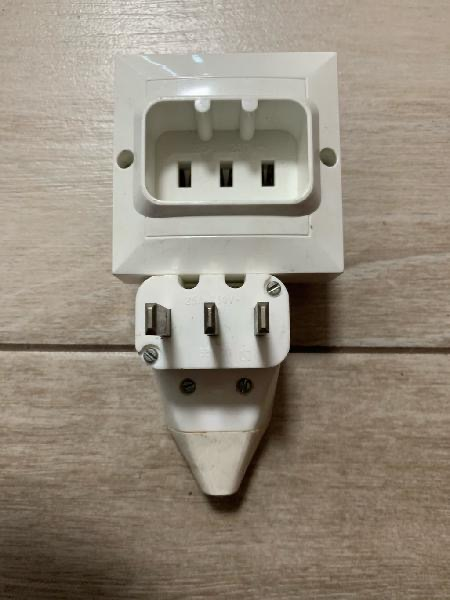
\includegraphics[scale=0.25]{chapters/0X_Normativas_02_MinimaLegal/25Aenchufe.jpg}

	\caption{Enchufes de 25A validos en España}
	\label{fig:25APared}
\end{figure}


De este enchufe de 25A nos podemos hacer nuestra propia caja de fusibles para la maqueta, y asi organizar como queramos los nuevos enchufes. En realidad nada nos impide hacernos nuestra caja de fusibles para 16A y poner interruptores, para iluminacion, DCC, accesorios,\dots

(Dibujo enchufe y caja fusible para la maqueta)

La ultima opcion es realizar una obra con profesionales indicando bien nuestras necesidades y ellos se encargen de todo.
\section{Discusión}
Como hemos dicho a nivel de peso sera dificil llegar al limite de nuestra casa para poner una maqueta, ya que por mucho que esta pese, siempre va a ser menor que una libreriria y ademas vamos a querer usar la mayor superficie posible.

Por otra parte en la parte electrica, hemos dicho que es un poco más complicado y que estamos juegando sobre seguro. En los ejemplos que hemos puesto habiamos dicho que la corriente alterna iba en una señal sinusoidal de 220V (o como mucho a 240V) y a este valor le aplicamos el factor de forma. Pero en realidad el valor de 220V es RMS\footnote{RMS: Root Median Square o Raiz cuadrada de la media}, o que es lo mismo aplicado el Factor de forma por lo que aun tenemos ese margen. Por ejemplo para una plancha, elemento resisitivo con factor de potencia 1, tenemos disponibles 3200W en un cable de 16A en vez de los 2500W que habiamos calculado previamente. 

Si quisieramos ser estrictos y trabajar sin el factor de forma de esos 3200W deberiamos quitar un margen de seguridad (al menos 10\%), luego aplicar un factor de potencia (que desconocemos, pongamos 75\%) y por ultimo el factor de eficiencia (pongamos unos 85\%), con estos datos temenos:

$3200W \cdot 90\% \cdot 75\% \cdot 85\% = 1836W $

Que es un poco mayor de los 1760 calculados previamente, siendo estos reales de salida (utlizables en maquinas) y con un 10% de margen para el error. 

Traducido en maquinas corriendo, con los calculos anteriores teniamos en el mejor de los casos 9 Boosters de 10 A haciendo un total de $180$ Maquinas.
Con este calculo tenemos $\frac{1836}{8}=229.5$ Maquinas disponibles. En ambos casos suponiendo 0,5 A por maquina y 16V.

Tampoco nos olvidemos de otras cosas que deben utilizar esos Watios, como son los accesorios (animaciones, desvios, iluminacion, paneles de control, mandos,...) pero estas cosas tan apenas consume:
\begin{itemize}
\item \textbf{Animaciones}: Los motores usados para  animaciones y los servos consumen muy poco unos 100ma cuando estan en uso, por lo que se necesitan 5 para alcanzar una maquina y su uso suele ser puntual, por lo que para que continuamente consuman como una maquina se necesitan mucho.

\item \textbf{Desvios}: Los desvios pueden usar servo motores, motores de animacion o sistemas de solenoides. En los dos primeros casos entrarian en el caso anterior, en el ultimo, utilizan mucha potencia cuando cambian pero es casi instantaneo y se usan CDUs que se cargan "lentamente" y seria igualemente un caso similar.

\item \textbf{Iluminacion}: Hoy en dia se usa los leds para iluminar diferentes elementos, un buen LED solo necesita 5mA para lucir brillantemente, uno malo 10mA por lo que una maquina pueden encender 50 leds, lo que da para los edificios de un pueblo tranquilamente. Si nos vamos a la iluminacion de la habitacion, aparte de que va por otro circuito, pero con 50W en lamparas de bajo consumo da de sobra, lo que son unas 5.1 maquinas (sobre 180...)

\item \textbf{Paneles de control y mandos}: Esto es lo que mas dificil de calcular, pero la mayoria son LEDs con botones.   
\end{itemize} 

\section{Conclusiones}
Hemos visto un par de normas que debemos tener en cuenta cuando hagamos nuestra maqueta. En general y para una maqueta domestica no debemos preocuparmnos mucho, pero si esta crece, o nos queremos construir una nueva habitacion estas normas las tendremos que tener en cuenta.



\section{Próximos pasos}

\section{Bibliografía}
\printbibliography[heading=subbibliography]
	
